\documentclass[tikz,border=12pt]{standalone}
\usepackage[T1]{fontenc}
\usepackage{mathpazo}
\usepackage{amsmath,amssymb}
\usetikzlibrary{arrows.meta, positioning, calc, fit, decorations.pathreplacing}

\definecolor{stblue}{HTML}{7B97AD}
\definecolor{rwgold}{HTML}{B8995E}
\definecolor{sage}{HTML}{7A9A7E}
\definecolor{dkbrown}{HTML}{3D3530}
\definecolor{wmgray}{HTML}{7B7067}
\definecolor{cream}{HTML}{F9F6F0}
\definecolor{border}{HTML}{D4C9B8}
\definecolor{terracotta}{HTML}{C47A6A}
\definecolor{lavender}{HTML}{907EA0}
\definecolor{rosefade}{HTML}{B56B6B}

\begin{document}
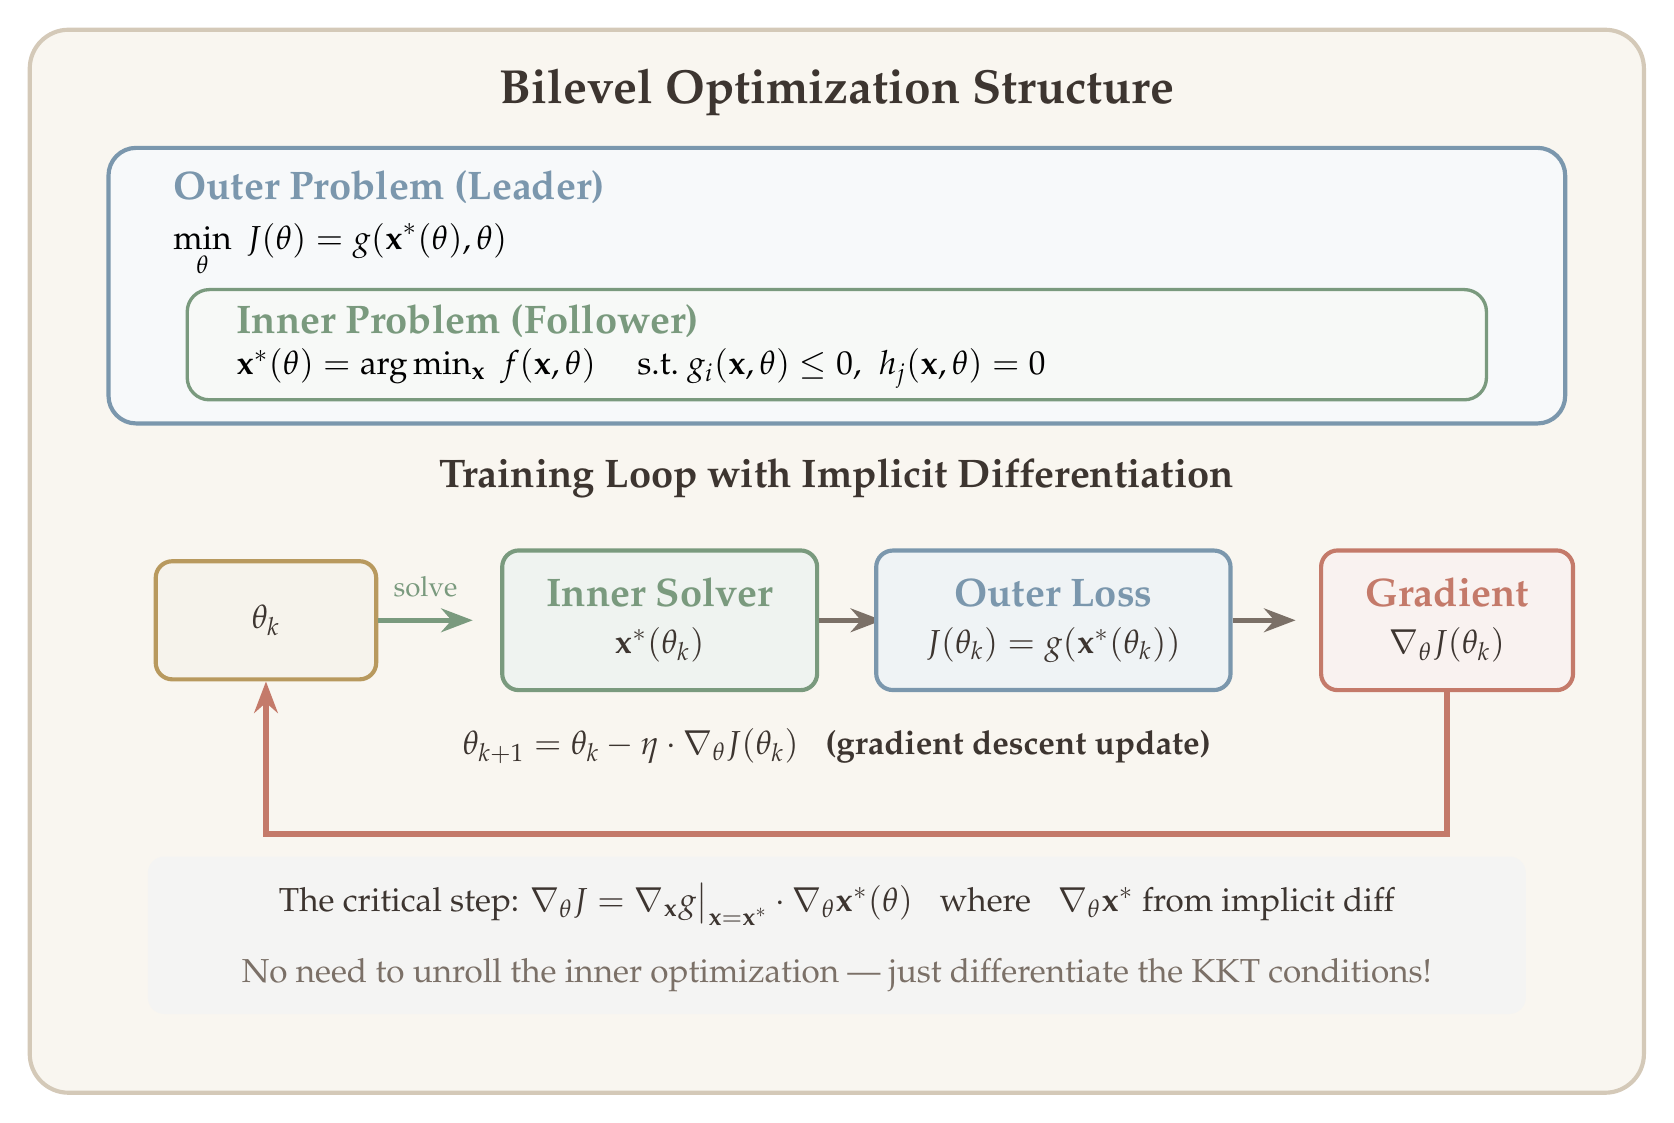
\begin{tikzpicture}[
  >={Stealth[length=4mm, width=3mm]},
  flowbox/.style={rounded corners=6pt, line width=1.5pt, minimum height=1.5cm,
                  align=center, text=dkbrown, font=\large, inner sep=10pt},
]

% Background
\fill[cream, rounded corners=14pt] (-0.5,-1) rectangle (20,12.5);
\draw[border, line width=1.5pt, rounded corners=14pt] (-0.5,-1) rectangle (20,12.5);

% Title
\node[font=\LARGE\bfseries, text=dkbrown] at (9.75,11.7) {Bilevel Optimization Structure};

% ============ Outer problem box ============
\draw[stblue, line width=1.5pt, rounded corners=10pt, fill=stblue!6]
  (0.5,7.5) rectangle (19,11);
\node[font=\Large\bfseries, text=stblue, anchor=west] at (1.2,10.5)
  {Outer Problem (Leader)};
\node[font=\large, anchor=west] at (1.2,9.7)
  {$\displaystyle\min_\theta\; J(\theta) = g(\mathbf{x}^*(\theta), \theta)$};

% Inner problem box (nested)
\draw[sage, line width=1.2pt, rounded corners=8pt, fill=sage!6]
  (1.5,7.8) rectangle (18,9.2);
\node[font=\Large\bfseries, text=sage, anchor=west] at (2.0,8.8)
  {Inner Problem (Follower)};
\node[font=\large, anchor=west] at (2.0,8.2)
  {$\mathbf{x}^*(\theta) = \arg\min_{\mathbf{x}}\; f(\mathbf{x}, \theta)$
   \quad s.t.\ $g_i(\mathbf{x}, \theta) \leq 0$, \;$h_j(\mathbf{x}, \theta) = 0$};

% ============ Training loop ============
\node[font=\Large\bfseries, text=dkbrown] at (9.75,6.8) {Training Loop with Implicit Differentiation};

% theta_k box
\node[flowbox, fill=rwgold!12, draw=rwgold, minimum width=2.8cm] (theta) at (2.5,5.0) {$\theta_k$};

% Arrow to inner solver
\draw[sage, line width=2pt, ->] (theta.east) -- ++(1.2,0)
  node[midway, above=4pt, font=\normalsize, text=sage] {solve};

% Inner solver box
\node[flowbox, fill=sage!12, draw=sage, minimum width=4.0cm] (solver) at (7.5,5.0) {%
  {\Large\bfseries\color{sage}Inner Solver}\\[3pt]
  $\mathbf{x}^*(\theta_k)$
};

% Arrow to outer loss
\draw[wmgray, line width=2pt, ->] (solver.east) -- ++(0.8,0);

% Outer objective box
\node[flowbox, fill=stblue!12, draw=stblue, minimum width=4.5cm] (outer) at (12.5,5.0) {%
  {\Large\bfseries\color{stblue}Outer Loss}\\[3pt]
  $J(\theta_k) = g(\mathbf{x}^*(\theta_k))$
};

% Arrow to gradient
\draw[wmgray, line width=2pt, ->] (outer.east) -- ++(0.8,0);

% Gradient box
\node[flowbox, fill=terracotta!10, draw=terracotta, minimum width=3.2cm] (grad) at (17.5,5.0) {%
  {\Large\bfseries\color{terracotta}Gradient}\\[3pt]
  $\nabla_\theta J(\theta_k)$
};

% Gradient descent update label (above the return arrow)
\node[font=\large\bfseries, text=dkbrown] at (9.75,3.4)
  {$\theta_{k+1} = \theta_k - \eta \cdot \nabla_\theta J(\theta_k)$ \;\;(gradient descent update)};

% Return arrow (below the label)
\draw[terracotta, line width=2pt, ->]
  (grad.south) -- ++(0,-1.8) -| (theta.south);

% Key computation annotation
\fill[wmgray!8, rounded corners=6pt] (1.0,0.0) rectangle (18.5,2.0);
\node[font=\large, text=dkbrown] at (9.75,1.4) {%
  The critical step: $\nabla_\theta J = \nabla_{\mathbf{x}} g\big|_{\mathbf{x}=\mathbf{x}^*} \cdot \nabla_\theta \mathbf{x}^*(\theta)$
  \;\;where\;\; $\nabla_\theta \mathbf{x}^*$ from implicit diff};
\node[font=\large, text=wmgray] at (9.75,0.5) {%
  No need to unroll the inner optimization --- just differentiate the KKT conditions!};

\end{tikzpicture}
\end{document}
